%% Beispiel-Präsentation mit LaTeX Beamer im KIT-Design
%% entsprechend den Gestaltungsrichtlinien vom Februar 2025
%%
%% Siehe https://sdq.kastel.kit.edu/wiki/Dokumentvorlagen

%% Beispiel-Präsentation
\documentclass{sdqbeamer} 
 
%% Gruppenlogo, muss im Verzeichnis logos/ liegen
%% falls kein Gruppenlogo gewünscht, bitte \grouplogo{} aufrufen
\grouplogo{} 

%% Gruppenname und Breite (Standard: 89 mm)
\groupname{Modelling for Continuous Software Engineering}
%\groupnamewidth{89mm}

% Beginn der Präsentation

\title[Automated Prompt Engineering for Traceability Link Recovery]{Automated Prompt Engineering for Traceability Link Recovery}
\subtitle{Bachelor's Thesis Proposal Presentation \\
Institute of Information Security and Dependability (KASTEL), Prof. Anne Koziolek \\
Modelling for Continuous Software Engineering (MCSE), Supervisor:  M.Sc. Dominik Fuchß} 
\author{Daniel Schwab}

\date[23.\,06.\,2025]{23. June 2025}

% Literatur 
 
\usepackage[citestyle=authoryear,bibstyle=numeric,hyperref,backend=biber]{biblatex}
\addbibresource{presentation.bib}
\bibhang1em

\usepackage{lipsum}
\usepackage{svg}
\usepackage{multirow}
\usepackage{tikz}
\usepackage{verbatim}
\usepackage{pgfgantt}

\begin{document}

%Titelseite
\begin{frame}[title white horizontal, picture=images/palladio_bauplan, kitlogo=white]
\titlepage
\end{frame}

%Inhaltsverzeichnis
%\begin{frame}[tableofcontents=green]{Inhaltsverzeichnis}
%	\tableofcontents
%\end{frame}


\section{Foundations}


\begin{frame}[picture 50 vertical, picture=images/artifact_overview_Fuchß.png]
\frametitle{What is Traceability Link Recovery (TLR)}
	\begin{itemize}
		\item Many artifacts are created during software development
            \item Often, inconsistencies will be present, such as naming
            \item Goal: Link elements across multiple domains or versions to ensure consistency and validation
            \item Image: Overview of possible artifacts for TLR by \cite{fuchss2025LiSSAGeneric}
	\end{itemize}
\end{frame}


\begin{frame}[picture 66 vertical, picture=images/iterative_core_loop.pdf]
\frametitle{What is Automated Prompt Engineering}
    \begin{itemize}
        \item Use the LLM to refine prompts instead of manually formulating them
        \item Improve initial prompt by training with a subset of the actual data
        \item Optimization prompt to fix previous shortcomings
    \end{itemize} 
\end{frame}

\begin{comment}
\begin{frame}
\frametitle{The LiSSA Framework}
    \begin{figure}
        \centering
        \includegraphics[width=0.9\linewidth]{images/LiSSA_pipeline_Fuchß.png}
        \caption{LiSSA pipeline by \cite{fuchss2025LiSSAGeneric}}
        \label{fig:enter-label}
    \end{figure}
    \begin{itemize}
        \item This work will add to the prompting step of the LiSSA framework
    \end{itemize}
    
\end{frame}
\end{comment}

\begin{frame}{Related Work}
    
    \begin{figure}
        \centering
        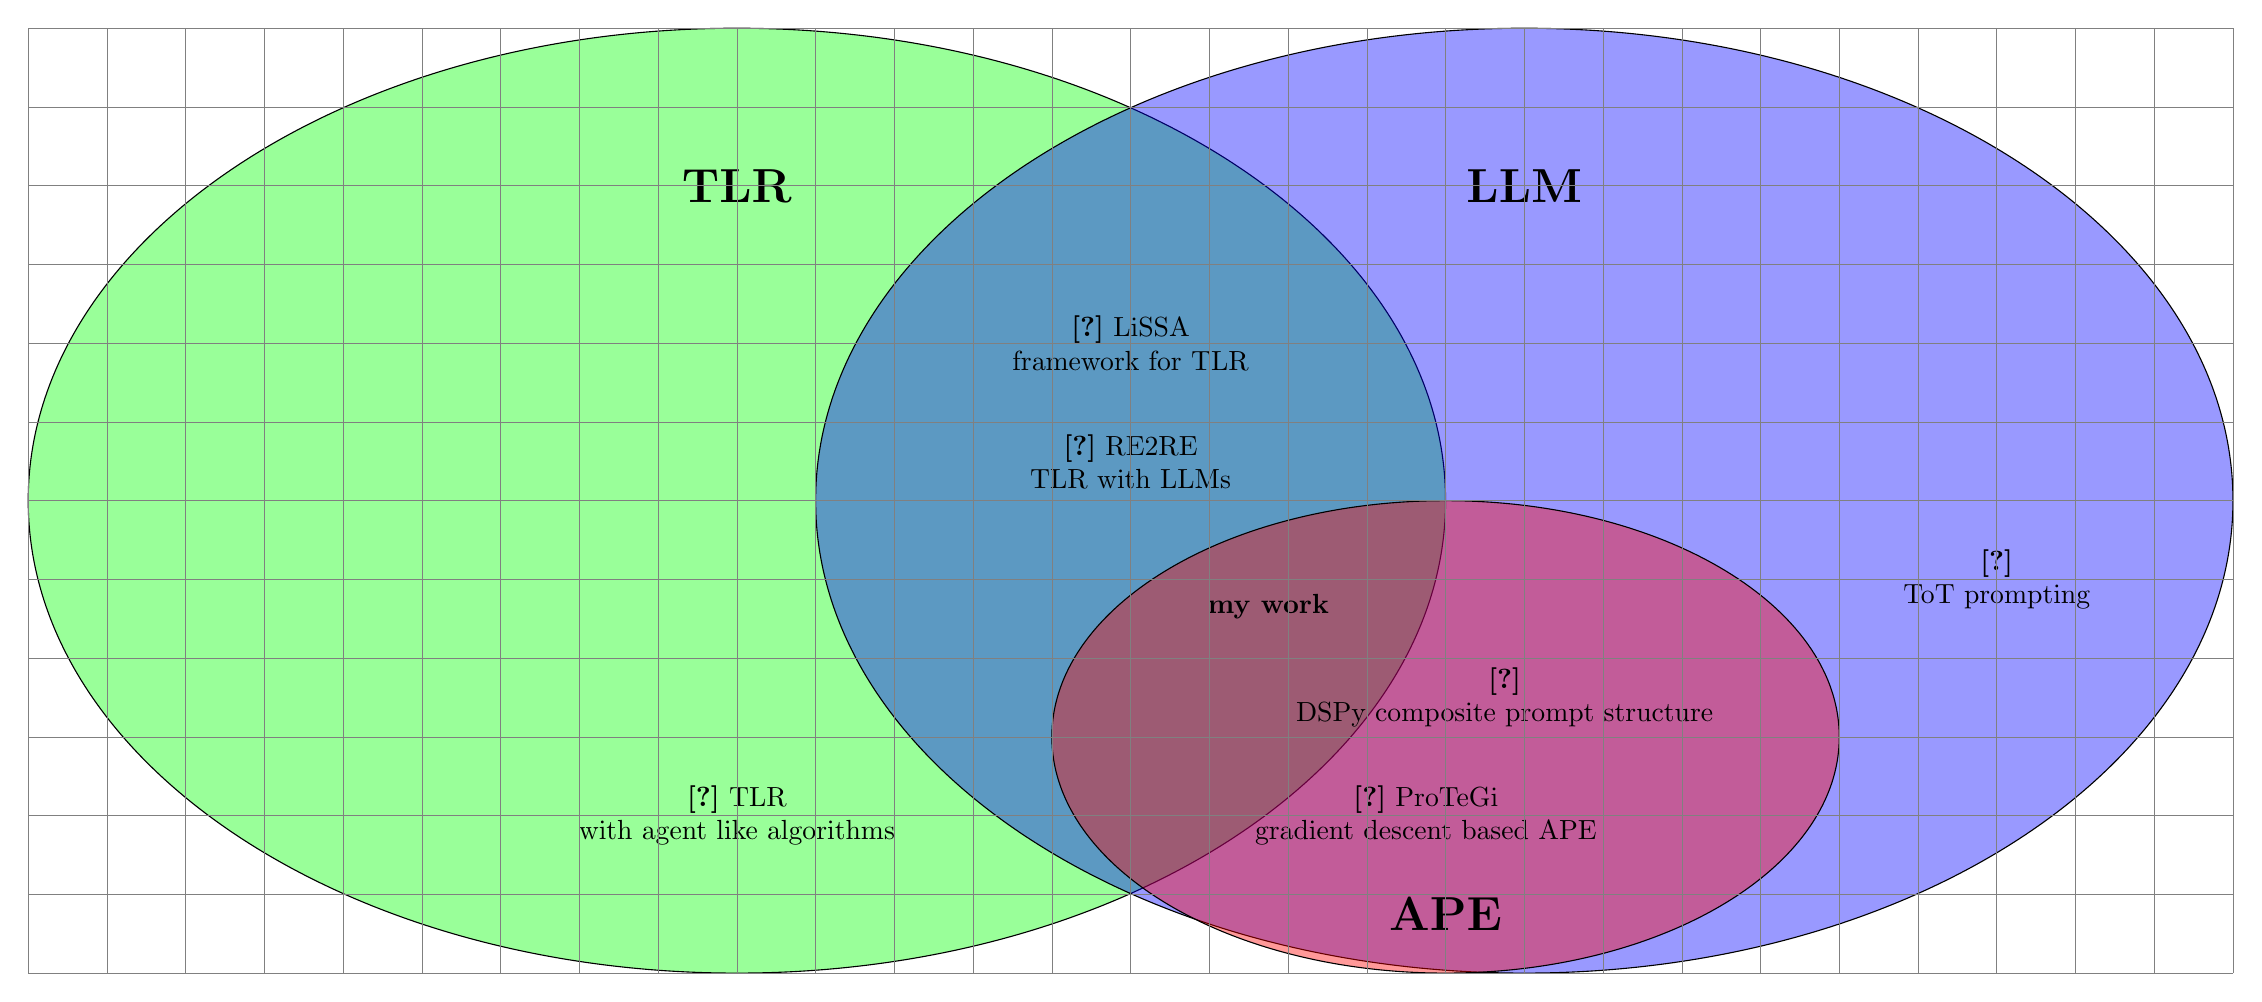
\begin{tikzpicture}
            \begin{scope} [fill opacity = .4, text opacity=1]
            \draw[fill=green, draw = black] (-5,0) ellipse (9 and 6);
            \draw[fill=blue, draw = black] (5,0) ellipse (9 and 6);
            \draw[fill=red, draw = black] (4,-3) ellipse (5 and 3);
            \node at (-5,4) {\LARGE\textbf{TLR}};
            \node at (5,4) {\LARGE\textbf{LLM}};
            \node at (4,-5.25) {\LARGE\textbf{APE}};
            \node[align=center] at (-5,-4) {\textbf{\cite{keim2021TraceLink}} TLR\\with agent like algorithms};

            %TLR with LLMs
            \node[align=center] at (0,0.5) {\textbf{\cite{hey2025RequirementsTraceability}} RE2RE\\TLR with LLMs};
            \node[align=center] at (0,2) {\textbf{\cite{fuchss2025LiSSAGeneric}} LiSSA\\framework for TLR};

            %LLM Work
            \node[align=center] at (11,-1) {\textbf{\cite{long2023LargeLanguage}} \\ToT prompting};

            %APE Work
            \node[align=center] at (4.75,-2.5) {\textbf{\cite{khattab2023DSPyCompiling}} \\DSPy composite prompt structure};
            \node[align=center] at (3.75,-4) {\textbf{\cite{pryzant2023AutomaticPrompt}}  ProTeGi\\gradient descent based APE};

            %Crosssection
            \node[align=center] at (1.75, -1.35) {\textbf{my work}};
            \end{scope}
        %% And now you have a venn diagram. Yay!
        \draw[help lines](-14,6) grid (14,-6);    
        \end{tikzpicture}
        \caption{Caption}
        \label{fig:enter-label}
    \end{figure}
    
\end{frame}


\section{Implementation}

\begin{frame}[picture 50 vertical, picture=images/gradient_descent.pdf]
\frametitle{Automated Prompt Engineering with Gradient Descent}
    \begin{itemize}
        \item Improved APE algorithm by \cite{pryzant2023AutomaticPrompt}
        \item Generate many new prompt candidates on each layer
        \item Steer them against the error direction using gradients
        \item Select the most promising candidates cheaply using a well-studied multiple-armed bandit algorithm
    \end{itemize}
    
\end{frame}


\section{Evaluation}

\begin{frame}{Evaluation}
    \begin{columns}
        \column{0.4\textwidth}{
            \begin{itemize}
                \item Compare performance (precision, recall, F1-score, F2-score) against current manually designed zero-shot and chain-of-thought prompt
                \item Apply variations of different initial prompts and different LLMs to the optimization problem and compare outputs
            \end{itemize}
        }
        \column{0.6\textwidth}{
            \begin{table}[]
                \centering
                \def\arraystretch{1.1}
                \begin{tabular}{c c | c c c}
                    \textbf{Dataset} & \textbf{Metric} & \textbf{IR only} & \textbf{KISS GPT-4o} & \textbf{CoT GPT-4o} \\
                    
                    \multirow{4}{*}{CCHIT} & P. & .198 & .234 & .367 \\
                    &  R. & .157 & .157 & .138 \\
                    & F1 & .175 & .188 & .200 \\
                    & F2 & .164 & .168 & .158 \\
                    \hline
    
                    \multirow{4}{*}{Dronology} & P. & .386 & .394 & .512 \\
                    & R. & .695 & .695 & .655 \\
                    & F1 & .497 & .503 & .575 \\
                    & F2 & .600 & .603 & .620 \\
                    \hline
                    \multirow{4}{*}{\parbox{4cm}{Average including datasets that are omitted in this table}} &  P. & .329 & .340 & .497 \\
                    & R. & .500 & .500 & .458 \\
                    & F1 & .387 & .401 & .451 \\
                    & F2 & .445 & .452 & .452 
                \end{tabular}
                \caption{Reduced results by \cite[Table 2]{hey2025RequirementsTraceability}}
                \label{tab:my_label}
            \end{table}
            
        }
    \end{columns}
    
\end{frame}

\section{Thesis Shedule}
\begin{frame}{Thesis Schedule}
    \ganttset{%
        calendar week text={%
            \currentweek
        }%
    }
    \begin{figure}
    \begin{center}
    \begin{ganttchart}[
    vgrid={*{6}{draw=none}, dotted},
    x unit=.14cm,
    y unit title=.8cm,
    y unit chart=.8cm,
    milestone left shift =-1,
    milestone right shift =1,
    time slot format=isodate,
    time slot format/start date=2025-06-23]{2025-06-23}{2025-10-26}
    \ganttset{bar height=.7}
        \gantttitlecalendar{year, month=name, week=26} \\
        \ganttgroup{Initial Overview}{2025-06-23}{2025-07-27} \\
        \ganttbar{LiSSA setup}{2025-06-23}{2025-07-06} \\
        \ganttbar{Tree of Thought implementation}{2025-07-07}{2025-07-13} \\
        \ganttbar[name=impl1]{Benchmark setup}{2025-07-21}{2025-08-03} \\
        \ganttgroup{Naive optimization}{2025-07-28}{2025-08-18} \\
        \ganttbar[name=impl2]{Iterative classifier}{2025-07-28}{2025-08-03} \\
        \ganttgroup{APE gradient descent}{2025-08-25}{2025-09-21} \\
        \ganttbar[name=impl3]{Implementation}{2025-08-25}{2025-09-10}\\

        
        \ganttgroup{Evaluation and Buffer}{2025-08-11}{2025-10-23} \\
        \ganttbar{Thesis writing}{2025-08-18}{2025-09-14} 
        \ganttbar{}{2025-09-29}{2025-10-11}
        \\
        
        \ganttbar[name=eval1]{Evaluation}{2025-08-11}{2025-08-24}
        \ganttbar[name=eval2]{}{2025-09-15}{2025-09-28}
    
        
    

        \ganttlink{impl1}{eval1}
        \ganttlink{impl2}{eval1}
        \ganttlink{impl3}{eval2}
      
    \end{ganttchart}
    %\caption{Gantt chart for thesis schedule}
    \end{center}
    \label{fig:gantt}
\end{figure}
\end{frame}


\appendix
\beginbackup

\begin{frame}[allowframebreaks]{Literatur}

\printbibliography
\end{frame}

%% ----------------------------------------
%% | /Test-Folie mit definierten Farben |
%% ----------------------------------------
\backupend

\end{document}
